\documentclass[a4paper,12pt,oneside]{report}
\usepackage{a4wide}
\usepackage{ucs}
\usepackage[utf8x]{inputenc}
\usepackage{xcolor}
\usepackage[czech,english]{babel}
\usepackage[pdftex, final]{graphicx}
\usepackage{alltt}
\usepackage{paralist}
\usepackage{mdwlist}
\usepackage{subfig}
\usepackage[final]{pdfpages}
\usepackage[final,pdftex, colorlinks=false]{hyperref}
\usepackage{fancyhdr}
%mensi mezera z figure
%\setlength{\belowcaptionskip}{-10pt}
\newcommand{\squeezeup}{\vspace{-2.5mm}}

\usepackage{url}


\usepackage{verbatim}
%\usepackage{pdfpages}
\usepackage{perpage} %the perpage package
%\MakePerPage{footnote} %the perpage package command

\usepackage{amsmath}
%\usepackage{hyperref}
\usepackage{acronym}
\usepackage[font=singlespacing]{caption}
\usepackage[font={small}]{caption}
\usepackage{multirow}
\usepackage{fancyvrb}
\usepackage{subfig}
\usepackage{titlesec}
\usepackage{listings}

\usepackage{footmisc}

\makeatletter
\def\verbatim@font{\linespread{1}\normalfont\ttfamily}
\makeatother

\usepackage{indentfirst}


%%%%%%%%%% zahlavi %%%%%%%%%%%






%cislovani kapitol
\renewcommand*\thesection{\arabic{section}}
\renewcommand{\chaptername}{}

%\titleformat{\chapter}{\normalfont\huge}{}{20pt}{\huge\textbf}

\renewcommand{\partname}{}
\renewcommand{\chaptername}{}




%Abstract
\usepackage{lipsum}
\newenvironment{abstractpage}
  {\cleardoublepage\vspace*{\fill}\thispagestyle{empty}}
  {\vfill\cleardoublepage}
\newenvironment{abstractx}[1]
  {\bigskip\selectlanguage{#1}%
   \begin{center}\bfseries\abstractname\end{center}}
  {\par\bigskip}








%%%%%%%%%%%% rozmery %%%%%%%%%%%%%%%%%%
\usepackage[%
%top=40mm,
%bottom=35mm,
%left=40mm,
%right=30mm
top=40mm,
bottom=35mm,
left=35mm,
right=25mm
]{geometry}


\renewcommand\baselinestretch{1.3}
\parskip=0.8ex plus 0.4ex minus 0.1 ex

%%%%%%%%%%%%%% Listings %%%%%%%%%%%%%%%%%

\definecolor{lightGrey}{RGB}{250,250,250}
\definecolor{darkGrey}{RGB}{230,230,230}
\lstdefinelanguage{psmap}
{morekeywords={scale, mapinfo, maploc, where, end, font, fontsize, color,
border, raster, width, paper,
vpoints, vareas, vlines, symbol, size, rgbcolumn, sizecolumn, cwidth,
rotatecolumn, },
morekeywords=[2]{y, n, none},
morecomment=[l]{\#},
}



\lstdefinestyle{script}{
    language=bash,
    basicstyle={\ttfamily\footnotesize},
    keywordstyle={\bfseries},
    commentstyle={\itshape},
    %frame=lines,
    backgroundcolor=\color{lightGrey}
}


\lstdefinestyle{mybash}{
   language=bash,
   basicstyle={\ttfamily},
   keywordstyle=[1]{\bfseries},
   keywordstyle=[2]{\color{black}},
   commentstyle={\itshape},
   %frame=lines,
   showstringspaces=false,
   backgroundcolor=\color{darkGrey},
}

\lstdefinestyle{python}{
   language=python,
   basicstyle={\ttfamily},
   keywordstyle=[1]{\bfseries},
   keywordstyle=[2]{\color{black}},
   commentstyle={\itshape},
   frame=lines,
   showstringspaces=false,
   backgroundcolor=\color{lightGrey},
}





%%%%%%%%%%%%%%%%%%%%%%%%%%%%%%%%%

\newcommand{\klicslova}[2]{\noindent\textbf{#1: }#2}
\newcommand{\modul}[1]{\emph{#1}}
%\newcommand{\instr}[1]{\lstinline[style=psmapInline]|#1|}
\author{Matěj Krejčí}
% \pagecolor{darkGrey}
\newcommand{\necislovana}[1]{%
\phantomsection
\addcontentsline{toc}{section}{#1}
\section*{#1}
\markboth{\uppercase{#1}}{}
}


%%%%%%%%%%%%%%%%%%%%%%%%%%%%%%
\begin{document}
\pagestyle{empty}




\renewcommand{\bibname}{Literatura}
\renewcommand{\contentsname}{Obsah}
\renewcommand{\figurename}{Obr.}
\renewcommand{\tablename}{Tab.}




%nastaveni velikosti footnote
\renewcommand\footnotelayout{\footnotesize}
\pagenumbering{gobble}


\begin{center}
%napisy
\newcommand{\napisCVUT}{Czech Technical University in Prague}
\newcommand{\napisFS}{Faculty of Civil Engineering}
\newcommand{\napisProgram}{Geodesy and Cartography}
\newcommand{\napisObor}{Geoinformatics}
\newcommand{\napisKatedra}{Department of Geomatics}
\newcommand{\napisVedouci}{Ing. Martin Landa, Ph.D.}
\newcommand{\napisAutor}{Bc. Matěj Krejčí}
\newcommand{\napisDatum}{Prague 2016}
\newcommand{\napisNazevI}{Processing of vector data using distributed}
\newcommand{\napisNazevII}{database systems in GIS}
\newcommand{\napisNazevAjI}{Využití distribuovaných databázových}
\newcommand{\napisNazevAjII}{ systémů pro správu vektorových dat v GIS}
\newcommand{\napisBakalarka}{Master thesis}
\newcommand{\napisPraha}{Prague 2016}
%
% prikazy
%\newcommand{\velka}[1]{\uppercase{#1}}
\newcommand{\velka}[1]{\textsc{#1}}
%
% 
\newif\ifpatitul
\patitultrue

\ifpatitul
{\Large\velka{\napisCVUT}}\\
\velka{\Large\napisFS}\\
\vfill
{\LARGE\velka{\napisBakalarka}}
\vfill
{\large\napisPraha\hfill\napisAutor}
\newpage
\fi%patitul


{\Large\velka{\napisCVUT}}\\
{\Large\velka{\napisFS}}\\
{\Large\velka{\napisProgram}}\\
{\Large\velka{\napisObor}}\\
\vfill
\includegraphics[width=3cm]{logo_cvut_cb} %~
\vfill

{\Large\velka{\napisBakalarka}}\\
{\Large\velka{\napisNazevI\\
\napisNazevII}}\\
{\large\velka{\napisNazevAjI\\
\napisNazevAjII}}
\vfill
{\large%
Supervisor: \napisVedouci\\
\napisKatedra\\
\bigskip
\napisDatum\hfill\napisAutor}
\end{center}

\newpage
\input{listsezadanim} % resi si zalomeni sam


\begin{abstractpage}
\begin{abstractx}{czech}

  CIL..


  \klicslova{Klíčová slova}{GIS, GRASS}
\end{abstractx}

\begin{abstractx}{english}

	Aim of...

  \klicslova{Keywords}{GIS, GRASS}
\end{abstractx}
\end{abstractpage}




\newpage
\newcommand{\odsaditodzhora}{\hskip1pt\vfill}

\odsaditodzhora
\noindent {\bf acknowledgment}

\vskip 1.5 \baselineskip



%%% ML: anglicky

\begin{flushleft}
\begin{tabular}{cp{0.3\textwidth}c}
V Praze dne .................
& 
&
..................................
\\
&&
(podpis autora)
\end{tabular}

\end{flushleft}
\newpage

\odsaditodzhora
\noindent {\bf Acknowledgment}

\vskip 1.5 \baselineskip

Thanks to God.
\newpage

\newpage

\tableofcontents


\newpage
\necislovana{Introduction}

\pagestyle{fancy}
\fancyhf{}
\renewcommand{\sectionmark}[1]{\markboth{#1}{}} % set the \leftmark
\fancyhead[L]{CTU in Prague}
\fancyhead[R]{\leftmark} % 1. sectionname
\fancyfoot[C]{\thepage}


\pagenumbering{arabic}
\setcounter{page}{1}
\subsection*{Context}
Over the years the capabilities of hard drives have increased massively and access speed too. According to study by International Data Corp, since 2007 we produce more data than we can store. This amount of data is widely named big data.
\subsection*{Motivation and contribution}

\subsection*{Aim of the thesis}

 



\newpage
\chapter*{Background of related work}\stepcounter{chapter}\addcontentsline{toc}{chapter}{Background of related work}
\paragraph*{Starter}

\section{Hadoop framework}
		\subsection*{Hadoop}
		 \emph{"The Apache Hadoop software library is a framework that allows for the distributed
		  processing of large data sets across clusters of computers using simple programming 
		  models. It is designed to scale up from single servers to 
		 thousands of machines, each offering local computation and storage. Rather than rely 
		 on hardware to deliver high-availability, the library itself is
		  designed to detect and handle failures at the application layer, so delivering a 
		  highly-available service on top of a cluster of computers,
		  each of which may be prone to failures."}
		\paragraph*{History}goes back to 2002 and the 
open-source project Apache Hadoop software for reliable, scalable,
distributed computing was launched. The project was originally
developed within Yahoo! company. That was the first company
which used framework Hadoop in production environments.

At the beginning of October 2003, Hadoop project was launched to improve performance
of the Apache Nutch web search engine in the short time (in January 2006) was moved to the new Hadoop sub project.
At around the same time  distributed file system called Google
file system, with the specific, permitting efficient and reliable access
the huge amount of data has been created. This abstract filesystem, widely called "user level"
filesystem runs as a service that is accessible via APIs and libraries. 
In 2008, Hadoop was made its own top-level project at Apache, confirming its
success and its diverse, active community. By this time, Hadoop was being used by many
other companies besides Yahoo!, such as Last.fm, Facebook, and the New York Times. 

\paragraph*{The base Apache Hadoop}framework \cite{apache_web} written in Java is composed of the following modules:
\begin{itemize}
\item \textbf{Hadoop Common} - The common utilities that support the other Hadoop modules;
\item \textbf{Hadoop Distributed File System (HDFS)} – A distributed file system that provides
 high-throughput access to application data;
\item \textbf{Hadoop YARN} - A framework for job scheduling and cluster resource management;
\item \textbf{Hadoop MapReduce} - an implementation of the MapReduce programming model 
for large scale data processing.
\end{itemize}
Beside main modules, there are many Hadoop extensions for cluster management, 
data access and helpers for storing data in HDFS.

		\subsection{HDFS: Hadoop Distributed File System}
		\paragraph*{Hadoop} comes with a filesystem and since it manages the storage of files across several machines, it is called Hadoop Distributed FileSystem (HDFS). Is designed for handling very large files with streaming
data access. In HDFS, large files are broken down into smaller blocks (128MB, by default) which are 
stored as independent units. The architecture of HDFS is a highly fault-tolerant and provides wide permeability
for access.   
  A short overview of main characteristics of HDFS design is described
 below\cite{hadoop_definitive}:
\begin{enumerate}
\item \textbf{Very large files} - With relevant hardware data of amounts petabites 
can be accessed on Hadoop clusters effectively.
\item \textbf{Streaming data access} - Efficient data processing is based on
 read once and copied many times pattern. 
\item \textbf{Commodity hardware} is suitable for running Hadoop. At the end,
 this fact helped with decision to invest value of money to the development of Hadoop instead 
 of operate on expensive and highly reliable hardware.
\item \textbf{Low-latency data access} - HDFS is not suitable for preforming
 low-latency access to data. Primary, HDFS is optimized for delivering
a high throughput of data.
\item \textbf{Lots of small files} allows to read and operate over more files
 at the same time. Limitation of number of stored directories,  files and block in filesystem is limited by \emph{Namenode} memory.

\begin{figure}[h!]
    \centering
    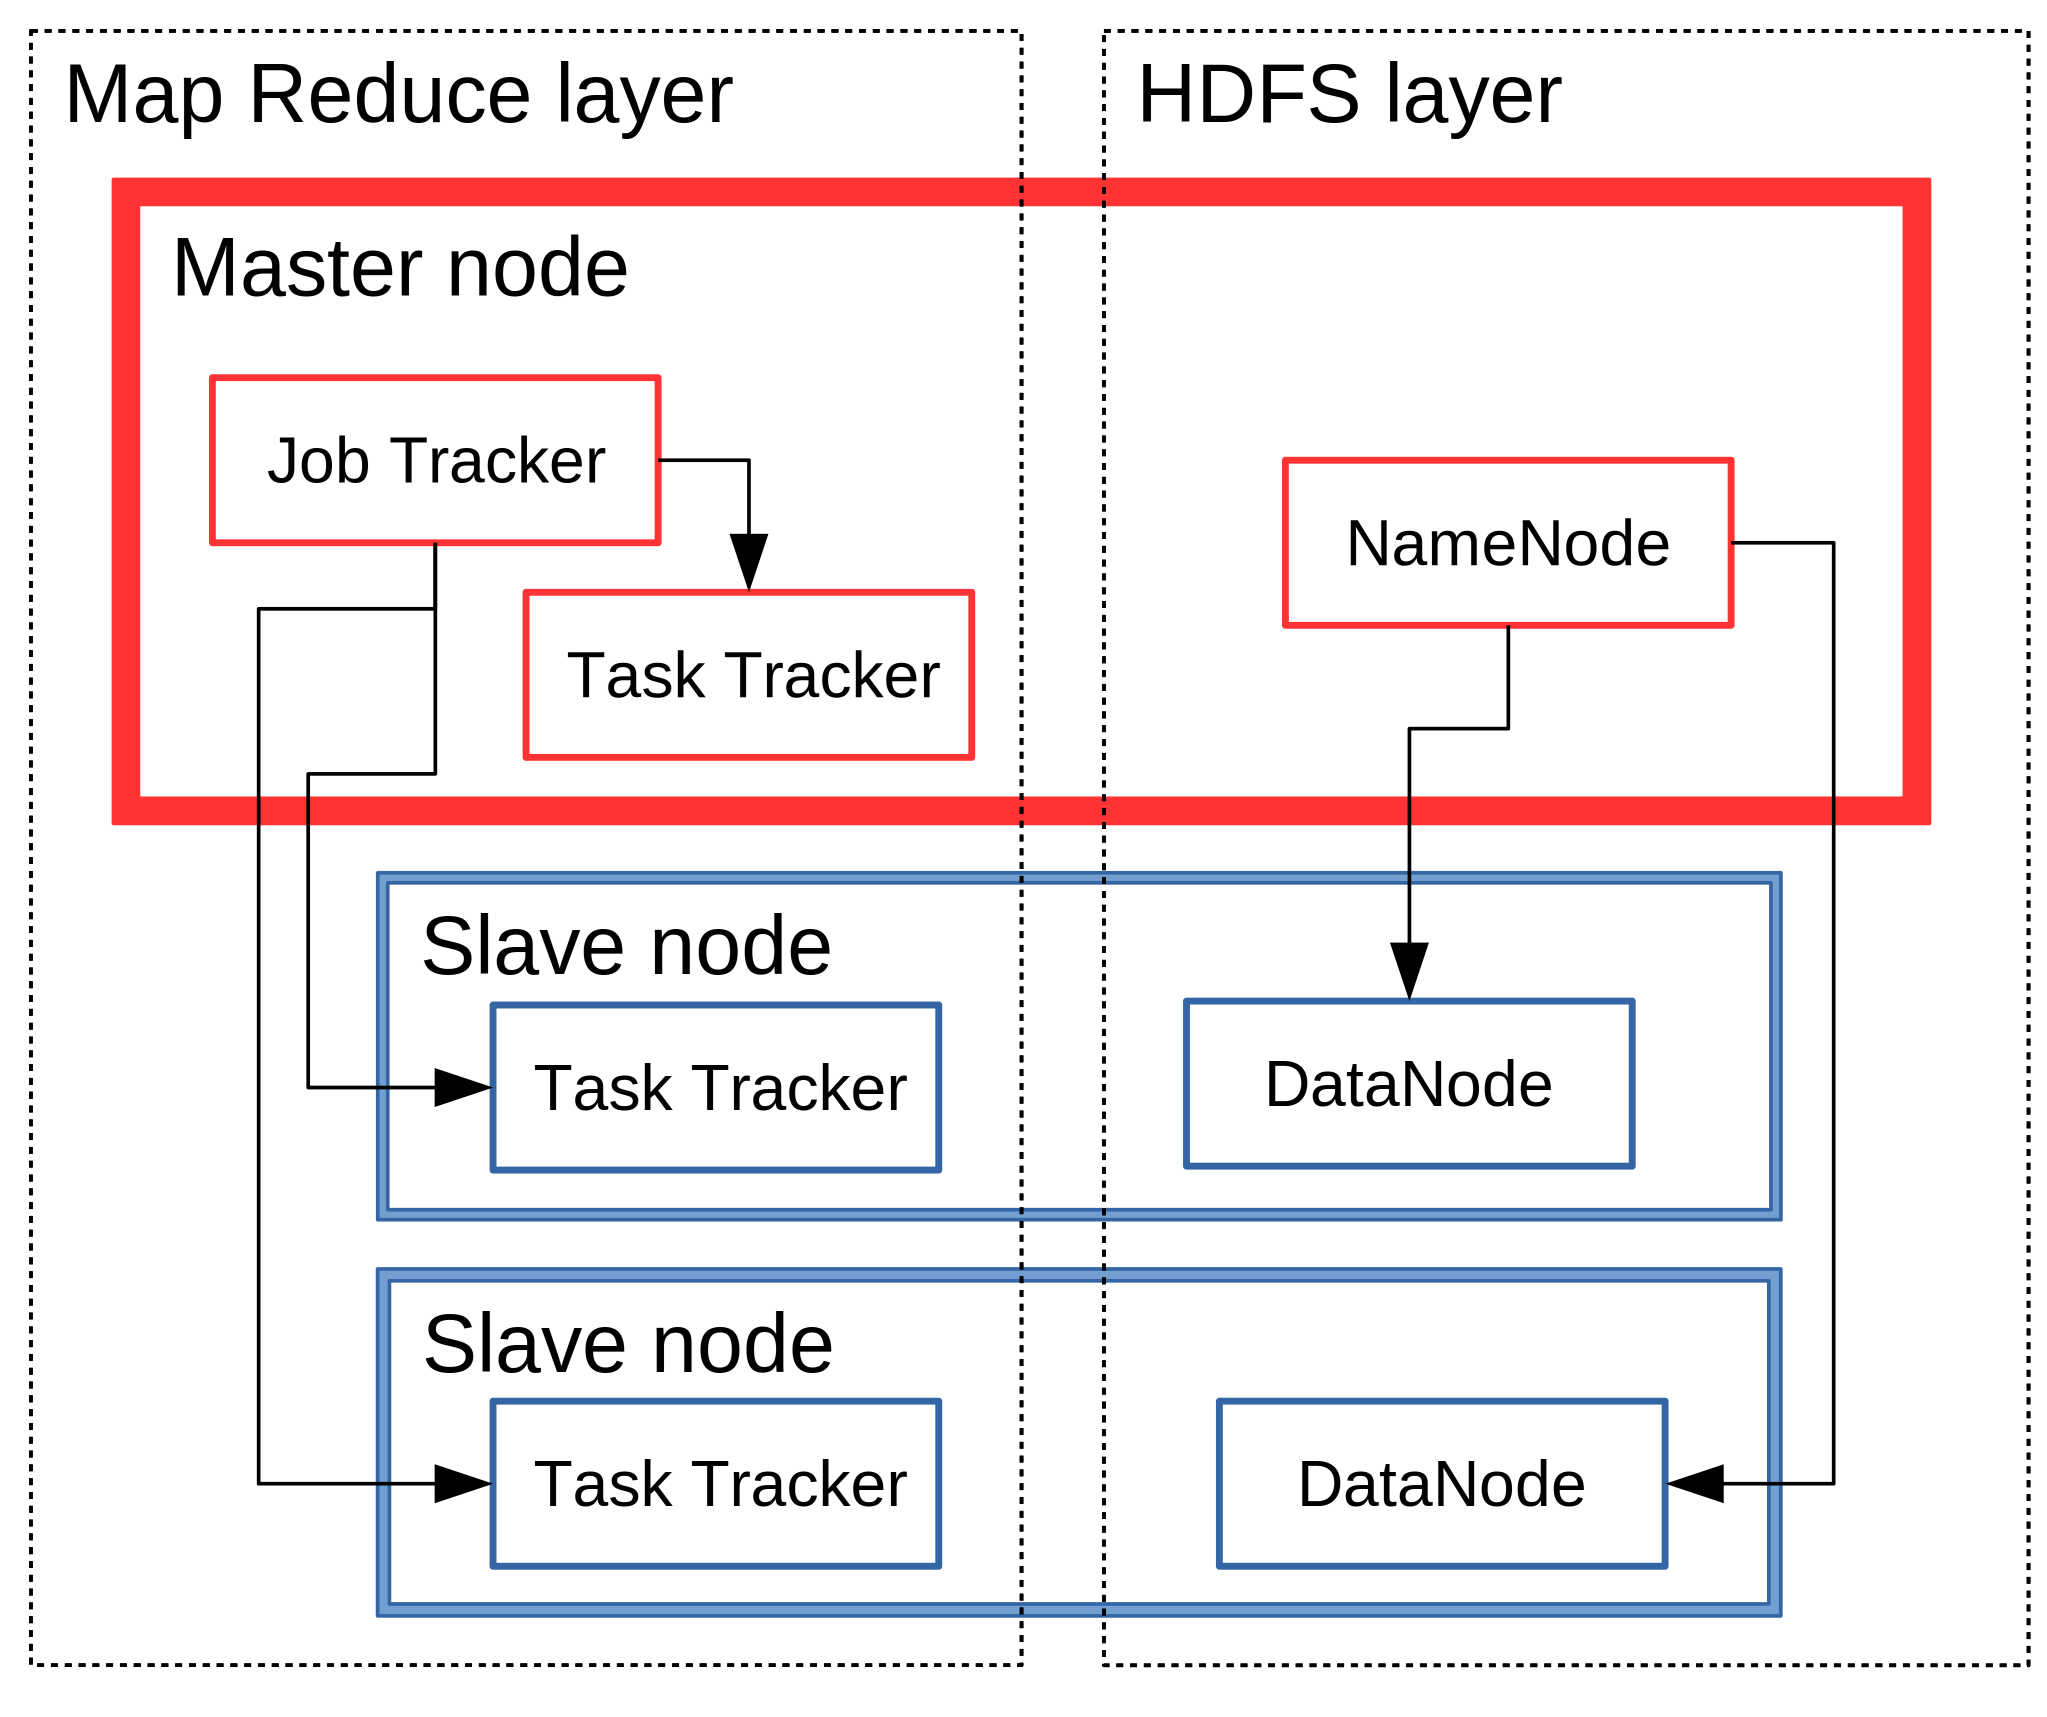
\includegraphics[width=0.6\textwidth]{./img/hadoop/schema2.pdf}
    \caption[Hadoop architecture]{\centering Hadoop architecture  }
 \end{figure} 
\end{enumerate}
		\subsubsection{Organisation of data}
Similarly to  a filesystem, HDFS as well is based on the disk blocks. The traditional
 the file system is based on blocks which define the minimal size of the amount of data to read and write. 
        HDFS blocks have the simillar concept based on blocks, but the minimal unit is
         large. The size of the block is 128 MB by default. Blocks are broken and distributed
          over disks on the cluster like blocks over a single disk in the filesystem. The ideal 
          size of stored files is the same as the size of the block. With increasing the block 
          size time cost for computing as well increasing.  On the other hand, a large number
           of blocks is expensive for the preparation of files. The important task is to find optimize 
            ratio between data preparation and computational time by set suitable blocks size.
        The idea of block abstraction helps to bring several benefits. First advantages of
         abstraction design is the possibility of storing bigger data file than physical disk unit, 
         even the fact that it is unusual.
        The second benefit of fixed size is simplifying storage management. Obviously is easy task
         to hold calculate size disponibility and eliminating metadata concerns(Is  not necessary 
         to store metadata of tree in data blocks, even in the same system.)
        Furthmore the blocks are suitable for replication for providing fault tolerance. Protection
         against corrupted blocks, disk or machines is based replication of block over a cluster. 
         To ensure the integrity of HDFS checksums when reading as well as reading data.
        
        
		

		\subsubsection{Namenodes}
Hadoop comes with cluster architecture based on master(\emph{Namenode}) and\\ slave(\emph{Datanode}) design pattern. 
        The \emph{Namenode} handles metadata of abstract file system(namespace), which include
        information about the structure of files and directories in the tree. Information about filesystem is stored 
        on local disk in two files: the namespace image and edit log file. 
        The \emph{Namenode} know all locations of  \emph{Datanodes} blocks where data 
        are stored. It also provides the primary user interface to access HDFS. 
        By design \emph{Namenode}  is a single point of failure and should be never overloaded and must be the most reliable node of the cluster.  Without \emph{Namenode}, HDFS is totally unserviceable. In recent Hadoop releases, there is also a backupnode- \emph{SecondaryNamenode}, always up to date with latest \emph{Namenode} status. It receives all the operations done by \emph{Namenode} and stores them in local memory. This permits to have the latest, up to date, namespace status when \emph{Namenode} fails. 
		\subsubsection{Datanodes}
As has been mentioned, the blocks of a file are independently stored in nodes, which are called
Datanodes. Every Datanode in the cluster makes registration process to the Namenode during starting. Besides that, each Datanode informs Namenode about blocks availability by sending a block report. A block reports are sent periodically or when a change event
happens. Moreover, every Datanode sends \emph{relevant} messages to the Namenode to confirm that
it remains operational and that the data is safe and available. If a Datanode stops operating, the error mechanisms designed to defend the failure and data loss maintain the availability of the block.
\emph{Relevant} messages also hold information, which allows the Namenode run the cluster efficiently e.g. load balancing.  One   important concept of design  is that Namenode never directly calls data.
		
		
		\subsubsection*{Data replication}
		\subsubsection*{I/O streams}

		
	\subsection{Parallel computing - MapReduce}		

The \emph{MapReduce} is a programming designed pattern for processing and generating large data
sets. The \emph{MapReduce} abstraction is inspired by the Map and Reduce functions, which is commonly
found in functional programming languages, such as LISP. Users can easily express their
computation as a series of Map and Reduce functions. The Map function processes a series of
\textit{$<$ key, value $>$} pairs to generate a set of intermediate \textit{$<$ key, value $>$} pairs.

\begin{center}
Map(keyA, valueA) → list (keyB, valueB)
\end{center}
Reduce function aggregates all intermediate values that associate to the same intermediate key
to produce the final output, also in the form of $<$ key, value $>$ pairs
\begin{center}
Reduce (keyB, list(valueB)) → list (key C, valueC)
\end{center}
Thus the \emph{MapReduce} framework transforms a list of (key, value) pairs into a list of values. 
%In this section the fundamentals of parallel computing with using Hadoop is described. 
%The basis of computing core is \emph{MapReduce} framework. As indicated, the \emph{MapReduce} consists two main 
%functions. After job is started the first function, \textbf{Map} is distributed over cluster of computers - in 
%Hadoop dialect over \emph{Datanodes}. 
%In \textbf{Map} function is defined form and location of reading row input data. According to character of 
%computation the pairs. The key is intermediate product and is stored locally.
%Reduce nodes take these intermediate outputs and using Reduce function combine them to final output which is then stored in HDFS.
%
%However, it essential that all the mapping function can run independently and their results can be proceeds by reducing 						function. Described principle allows almost linearly parallelizable solution of task.


\paragraph{As MapReduce demonstration} for this work is suitable to use we data from cellular microwaves links(MWL). 
Assume that data are already serialized and stored in text files. Each file representing 24 hours of captured data. 
Size amount of weakly data is relatively small(~100Mb) which is suitable.
We are interesting to compute mean of difference between transmitted and received signal
 for each link in period between 2014-07-07 and 2015-07-07.

Below is sample of data stored as CSV.
\begin{figure}[h!]
\begin{footnotesize}
\lstset{extendedchars=false,
escapeinside=''}
\begin{lstlisting}[style=mybash]
linkid;data;rx;tx
324;"2014-07-07 11:14:56.552";-48.9;10
256;"2014-07-07 11:14:59.703";-99.9;7
...
324;"2015-07-07 17:10:56.578";-50.1;7;
256;"2015-07-07 17:10:56.484";-85.3;10;
\end{lstlisting}
\end{footnotesize} 
\end{figure}

The lines above are presented to map functions as key-values pairs.
The map function extracts data from date 2014-07-07 and creates pairs {link:(rx-tx)}

\begin{figure}[h!]
\begin{footnotesize}
\lstset{extendedchars=false,
escapeinside=''}
\begin{lstlisting}[style=mybash]
{324:-58.9}
{256:-106.9}
...
{324:-57.1}
{256:-95.3}
\end{lstlisting}
\end{footnotesize} 
\end{figure}
The output is processed by MapReduce framework before is being sent to reduce function.
 Mentioned process sorts pairs by key as bellow.
\begin{figure}[h!]
\begin{footnotesize}
\lstset{extendedchars=false,
escapeinside=''}
\begin{lstlisting}[style=mybash]
{324:[-58.9,-57.1]}
{256:[-106.9,-95.3]}
\end{lstlisting}
\end{footnotesize} 
\end{figure}
Finally reduce program iterate over the list of values for each link and compute mean.
 The final results are stored in Hadoop file system.
%	    \subsection{Running MapReduce task}
%\begin{itemize}
%  \item[1] Client program uploads files to the Hadoop Distributed File System (HDFS) location and notifies the JobTracker which in turn returns the Job ID to the client.
%The Jobtracker allocates map tasks to the TaskTrackers..
%  \item[2] The JobTracker will first determine the number of splits (each split is configurable, ~16-64MB) from the input path, and select some TaskTracker based on their network proximity to the data sources, then the JobTracker send the task requests to those selected TaskTrackers.
%  \item[3 M] JobTracker determines appropriate jobs based on how busy the TaskTracker is.
%  \item[4 M] Each TaskTracker will start the map phase processing by extracting the input data from the splits. For each record parsed by the “InputFormat”, it invoke the user provided “map” function, which emits a number of key/value pair in the memory buffer. A periodic wakeup process will sort the memory buffer into different reducer node by invoke the “combine” function. The key/value pairs are sorted into one of the R local files (suppose there are R reducer nodes).
%  \item[5 M]The buffer is eventually flushed into two files.
%  \item[6 M]When the map task completes (all splits are done), the TaskTracker will notify the JobTracker. When all the TaskTrackers are done, the JobTracker will notify the selected TaskTrackers for the reduce phase.
%  \item[6 M]Each TaskTracker will read the region files remotely. It sorts the key/value pairs and for each key, it invoke the “reduce” function, which collects the key/aggregatedValue into the output file (one per reducer node).
%  
%Map/Reduce framework is resilient to crash of any components. The JobTracker keep tracks of the progress of each phases and periodically ping the TaskTracker for their health status. When any of the map phase TaskTracker crashes, the JobTracker will reassign the map task to a different TaskTracker node, which will rerun all the assigned splits. If the reduce phase TaskTracker crashes, the JobTracker will rerun the reduce at a different TaskTracker.
%  
%  When the map task completes (all splits are done), the TaskTracker will notify the JobTracker. When all the TaskTrackers are done, the JobTracker will notify the selected TaskTrackers for the reduce phase.
%\begin{figure}[h!]
%    \centering
%    \includegraphics[width=1\textwidth]{./img/hadoop/MapReduce.png}
%    \caption[Logo PostgreSQL]{\centering Logo PostgreSQL }
% \end{figure}   
	
	\subsection{Execution workflow}

The MapReduce framework splits the input files in to \emph{M} pieces of typically 16 to 128
megabytes (MB) per piece. It then starts many copies of the program on a cluster, including 1
\emph{Namenode} and other \emph{Datanode}. The \emph{Namenode}  is responsible for scheduling the job to each
\emph{Datanode}, and monitoring the job progress and \emph{Datanode’s} health.
\emph{Datanode} with are asking to \emph{Namenode} tasks of certain types (Map
or Reduce, or both). The \emph{Namenode} is checking the pool of non-running (including failed) tasks
and assign one or more tasks to the Worker. Map tasks are assigned with priority to
data locality. When a \emph{Datanode} is assigned with a Map task, it first reads the content of the
corresponding input split (either locally or remotely) and emits $<$ key, value $>$ pairs to the
user-defined Map function.
\begin{figure}[h!]
    \centering
    \includegraphics[width=1\textwidth]{./img/hadoop/map_reduce_architecture.png}
    \caption[mapreduce flow]{\centering Running MapReduce job}
 \end{figure} 
The output of the Map function is first buffered in the memory and periodically written
to local disks. A partitioning function partitions the output into \emph{R} sets, each associated with
a Reducer task The \emph{Namenode} passes the location of these outputs to \emph{Datanode’s} with Reduce tasks
running, which read these buffered data. The Reduce task
then sorts all the intermediate keys so that occurrences of the same key are grouped together.
For each key, the entire list of values is passed to the Reduce function. Each Reducer, upon
finishing its share of keys, outputs a result file (R output files in total).

\section{Distributed spatial data}
		\subsection{Serialization/De-serialization}
		\subsection{Spatial indexing and analytic on Hadoop}
		\subsection{Project: Spatial framework for Hadoop}
			\subsubsection{Java geometry API}

\section{Technologies Behind}
	\subsection{Spatial framework GRASS GIS}
		\paragraph*{Postgis driver}
	\subsection{Data warehouse: Hive}
		\paragraph{About}
		\subsubsection{Performance limitation}
	\subsection{Cluster virtualisation}
		\subsubsection{Docker}
		\subsubsection{Google cloud services}
		
		


	
\newpage
\chapter*{Experiment framework}\stepcounter{chapter}\addcontentsline{toc}{chapter}{Practical framework}


\setcounter{footnote}{1}
\newpage
\necislovana{Conclusion}



\pagenumbering{gobble}
\newpage
\necislovana{Seznam použitých zkratek}
\begin{acronym}
 \setlength{\parskip}{0ex}
 \setlength{\itemsep}{1ex}
  	\acro{API}{Application Programming Interface}
  	\acro{CSV}{Comma Separated Values}

  	\acro{EPSG}{Geodetic Parameter Set}	
  	
  	\acro{GIS}{Geographic Information System}
  	\acro{GNU GPL}{GNU General Public License } 
	\acro{GRASS}{Geographical Resources Analysis Support System}
	\acro{GUI}{Graphical User Interface}

\end{acronym}





\newpage
\renewcommand\baselinestretch{1.2}
\selectfont
\renewcommand{\refname}{Sources}
\phantomsection
\addcontentsline{toc}{section}{ \refname}

\begin{thebibliography}{99}
\label{literatura}




\bibitem{radar_meterology}
RAGHAVAN, S. \textit {Radar meteorology}.
31 Oct 2003. Boston: Kluwer Academic Publishers, 2003, 549 s. ISBN 14-020-1604-2. 


%\bibitem{coppock}
%COPPOCK J.T.,  RHIND D.W. \textit{The History of GIS}
%In Maguire D.J., Goodchild M.F., and Rhind D.W. (editors) Geographical Information Systems : Principles and Applications, 1991, Volume 1
%
%\bibitem{neuman}
%NEBEKER, Frederik. \textit{Calculating the weather: meteorology in the 20th century}
% San Diego: Academic Press, c1995, vii, 255 p. ISBN 01-251-5175-6. 
%
%\bibitem{slavicek}
%SLAVÍČEK, Marek. \textit{Zkoumání srážkoodtokových vztahů v urbanizovaném územi}
% Praha, 2003. Disertační práce Ph.D. ČVUT.
%
%
%\bibitem{wpc}
%Hydrometeorological Prediction Center \textit{ A Brief History of the Hydrometeorological Prediction Center}
%[cit. 2014-04-14] URL: \textless\url{ http://www.hpc.ncep.noaa.gov/html/WPC_history.pdf}$>$
%
%
%\bibitem{flash_floods}
%SENE, Kevin. \textit {Flash floods forecasting and warning}.
%2013. Dordrecht: Springer, 2013. ISBN 978-940-0751-644. 



\end{thebibliography}




\setcounter{footnote}{1}
\newpage



\appendix
\chapter*{Attachment}
\renewcommand\thesection{\Alph{section}}



\end{document}









